\usetikzlibrary{arrows.meta,patterns}

\begin{frame}{is there enough empty space?}
\begin{itemize}
    \item cavities look awfully small
    \item really small viruses?
    \item solution: chain cavities tgoether
\end{itemize}
\end{frame}

\begin{frame}{case study: CIH (1)}
    \pdftooltip{
    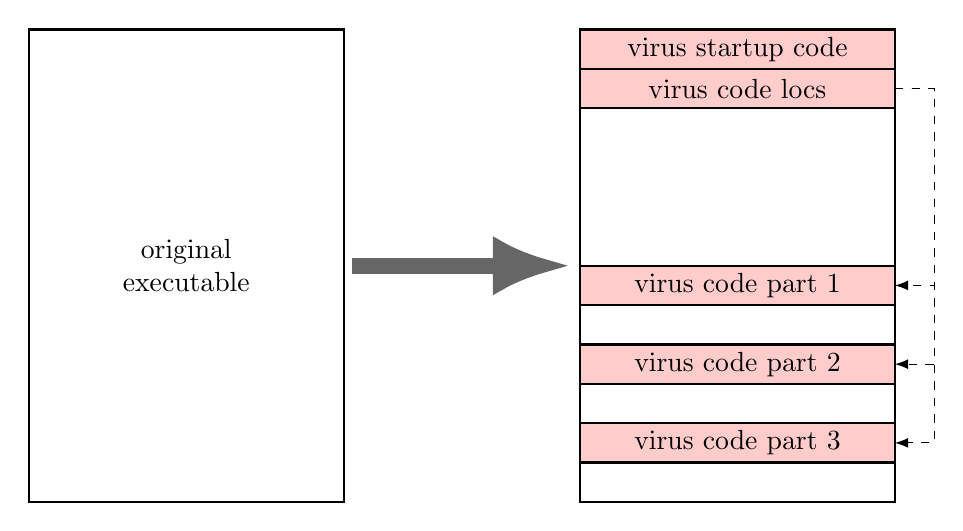
\begin{tikzpicture}
    \draw[thick] (0, 0) rectangle (4, -6) node[midway,align=center] {original\\executable};
    \draw[line width=2mm,-Latex,black!60] (4.1, -3) -- (6.9, -3);
    \begin{scope}[xshift=7cm]
    \draw[fill=red!20,thick] (0, 0) rectangle (4, -0.5) node[midway] {virus startup code};
    \draw[fill=red!20,thick] (0, -0.5) rectangle (4, -1) node[midway] {virus code locs};
    \draw[thick] (0, -1) rectangle (4, -6);
    \draw[fill=red!20,thick] (0, -3) rectangle (4, -3.5)
        node[midway] {virus code part 1};
    \draw[fill=red!20,thick] (0, -4) rectangle (4, -4.5)
        node[midway] {virus code part 2};
    \draw[fill=red!20,thick] (0, -5) rectangle (4, -5.5)
        node[midway] {virus code part 3};
    \draw[dashed,thin,-Latex] (4, -0.75) -- (4.5, -0.75) |- (4, -3.25);
    \draw[dashed,thin,-Latex] (4, -0.75) -- (4.5, -0.75) |- (4, -4.25);
    \draw[dashed,thin,-Latex] (4, -0.75) -- (4.5, -0.75) |- (4, -5.25);
    \end{scope}
    \end{tikzpicture}
    }{
        original excutable is transformed to contain virus startup code followed by
        a table of virus code locations.
        Most of the virus code is in the locations pointed to by the table, which were cavaties.
    }
\end{frame}

\begin{frame}{case study: CIH (2)}
    \pdftooltip{
    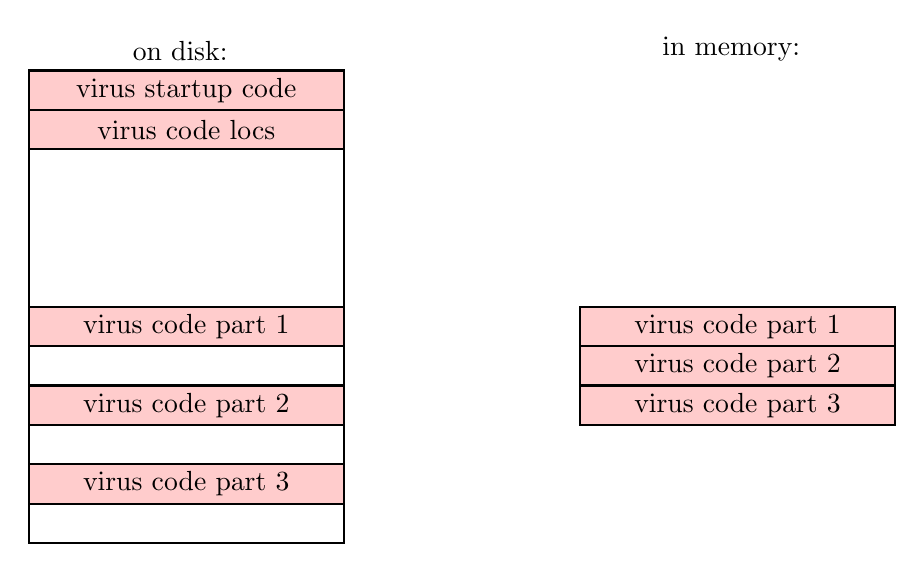
\begin{tikzpicture}
        \node[align=center,anchor=south] at (2, 0) { on disk: };
    \draw[fill=red!20,thick] (0, 0) rectangle (4, -0.5) node[midway] {virus startup code};
    \draw[fill=red!20,thick] (0, -0.5) rectangle (4, -1) node[midway] {virus code locs};
    \draw[thick] (0, -1) rectangle (4, -6);
    \draw[fill=red!20,thick] (0, -3) rectangle (4, -3.5)
        node[midway] {virus code part 1};
    \draw[fill=red!20,thick] (0, -4) rectangle (4, -4.5)
        node[midway] {virus code part 2};
    \draw[fill=red!20,thick] (0, -5) rectangle (4, -5.5)
        node[midway] {virus code part 3};
    \begin{scope}[xshift=7cm]
        \node[align=center,anchor=south] at (2, 0) { in memory: };
        \draw[fill=red!20,thick] (0, -3) rectangle (4, -3.5)
            node[midway] {virus code part 1};
        \draw[fill=red!20,thick] (0, -3.5) rectangle (4, -4)
            node[midway] {virus code part 2};
        \draw[fill=red!20,thick] (0, -4) rectangle (4, -4.5)
            node[midway] {virus code part 3};
    \end{scope}
    \end{tikzpicture}
    }{
        When the virus runs, the virus code parts are copied into contiguous storage before
        running.
        This alllows them to run without dealing worrying about whether instructions were
        split into two pieces or about inserting jumps between the parts of the virus code.
    }
\end{frame}

\begin{frame}{CIH cavities}
    \begin{itemize}
    \item gaps between sections
        \begin{itemize}
        \item common Windows linker aligned sections
        \item (align = start on address multiple of $N$, e.g. $4096$)
        \end{itemize}
    \item reassembling code avoids worrying about splitting instructions
    \end{itemize}
\end{frame}

